\documentclass[10pt]{beamer}
\usefonttheme{professionalfonts,serif}
\def\newblock{\hskip .11em plus .33em minus .07em}
\usepackage[numbers,sort]{natbib}
\renewcommand{\rmdefault}{psbx}
\usepackage[utf8]{inputenc}
\usepackage[T1]{fontenc}
\usepackage{textcomp}
\usepackage{eulervm}

\usetheme{default}           % tips from David Blei
\useinnertheme{circles}
\useoutertheme{infolines}
\setbeamertemplate{headline}{}
\setbeamertemplate{navigation symbols}{}
\setbeamerfont{itemize/enumerate subbody}{size=\normalsize}
\setbeamerfont{itemize/enumerate subsubbody}{size=\normalsize}
\usecolortheme{seahorse}
\setbeamersize{text margin left=2mm,text margin right=2mm}

\graphicspath{{../../figures/}}

\definecolor{mypine}{rgb}{0.05,0.45,0.05}
\definecolor{mycyan}{rgb}{0.0,0.9,0.9}
\newcommand{\Red}{\textcolor{red}}
\newcommand{\Blue}{\textcolor{blue}}
\newcommand{\Green}{\textcolor{mypine}}
\newcommand{\PineGreen}{\textcolor{mypine}}
\newcommand{\Magenta}{\textcolor{magenta}}
\newcommand{\Cyan}{\textcolor{mycyan}}

\newcommand{\N}{\mathcal{N}}
\newcommand{\R}{\mathbb{R}}
\newcommand{\T}{{\scriptsize^{\top}}}
\newcommand{\D}{\mathcal{D}}
\newcommand{\F}{\mathcal{F}}
\newcommand{\E}{\mathbb{E}}
\newcommand{\V}{\mathbb{V}}
\newcommand{\M}{\mathcal{M}}
\newcommand{\KL}{\mathcal{KL}}
\newcommand{\cut}[1]{}
\newcommand{\trace}{\operatorname{trace}}

\newcommand{\bmu}{{\boldsymbol{\mu}}}
\newcommand{\btheta}{\boldsymbol{\theta}}
\newcommand{\bepsilon}{\boldsymbol{\epsilon}}
\newcommand{\balpha}{\boldsymbol{\alpha}}
\newcommand{\bbeta}{\boldsymbol{\beta}}
\newcommand{\bphi}{\boldsymbol{\phi}}
\newcommand{\bPhi}{\boldsymbol{\Phi}}
\newcommand{\bSigma}{\boldsymbol{\Sigma}}
\newcommand{\bpi}{\boldsymbol{\pi}}
\newcommand{\blambda}{\boldsymbol{\lambda}}

\newcommand{\argmax}{\operatorname{argmax}}
\newcommand{\argmin}{\operatorname{argmin}}
\newcommand{\ci}{{\bot\negthickspace\negthickspace\bot}} % conditional indep.
\newcommand{\neigh}{\operatorname{ne}}
\newcommand{\vectr}[2]{  \left[ \!\!\begin{array}{c} #1 \\
      #2 \end{array} \!\!\right]}
\newcommand{\deff}{\stackrel{\mathrm{def}}{=}}
\newcommand{\deldel}[2]{\frac{\partial #1}{\partial #2}}

\newcommand{\maketilde}{\raisebox{0.4ex}{\tiny $\sim$}}
\newcommand{\bfa}{\mathbf a}
\newcommand{\bfb}{\mathbf b}
\newcommand{\bfe}{\mathbf e}
\newcommand{\bff}{\mathbf f}
\newcommand{\bfk}{\mathbf k}
\newcommand{\bfm}{\mathbf m}
\newcommand{\bfn}{\mathbf n}
\newcommand{\bfp}{\mathbf{p}}
\newcommand{\bfs}{\mathbf s}
\newcommand{\bfu}{\mathbf u}
\newcommand{\bfx}{\mathbf x}
\newcommand{\bfy}{\mathbf y}
\newcommand{\bft}{\mathbf t}
\newcommand{\bfv}{\mathbf v}
\newcommand{\bfw}{\mathbf w}
\newcommand{\bfA}{\mathbf A}
\newcommand{\bfI}{\mathbf I}
\newcommand{\bfK}{\mathbf K}


\title{Posterior Gaussian Process}
\author{Carl Edward Rasmussen}
\date{October 13th, 2016}

\begin{document}

\begin{frame}
\titlepage
\end{frame}

\begin{frame}
\frametitle{Key concepts}
\begin{itemize}
\item we are not interested in random functions
\item we want to \emph{condition} on the training data
\item when both prior and likelihood are Gaussian, then
\begin{itemize}
\item posterior is a Gaussian process
\item predictive distributions are Gaussian
\end{itemize}
\item pictorial representation of prior and posterior
\item interpretation of predictive equations
\end{itemize}
\end{frame}

\begin{frame}
\frametitle{Gaussian Process Inference}

Recall Bayesian inference in a parametric model.\\[1ex]

The posterior is proportional to the prior times the likelihood.\\[1ex]

The predictive distribution is the predictions marginalized over the
parameters.\\[1ex]

How does this work in a Gaussian Process model?\\[1ex]

Answer: in our non-parametric model, the ``parameters'' are the function itself!
\end{frame}


\begin{frame}
\frametitle{Non-parametric Gaussian process models}

In our non-parametric model, the ``parameters'' are the function itself!

Gaussian likelihood, with noise variance $\sigma_{\rm noise}^2$
\[
\Red{p({\bf y}|{\bf x}, f, \mathcal{M}_i)\;\sim\;
{\cal N}({\bf f},\;\sigma^2_{\rm noise}I),}
\]

Gaussian process prior with zero mean and covariance function $k$
\[
\Blue{p(f|\mathcal{M}_i)\;\sim\;{\cal GP}(m\equiv 0,\;k),}
\]

Leads to a Gaussian process posterior
\[
\begin{split}
\Green{p(f}&\Green{|{\bf x},{\bf y}, \mathcal{M}_i)\;\sim\;{\cal
    GP}(m_{\rm post},\;k_{\rm post}),}\\
&\text{where}\left\{\begin{array}{l}\!\!\Green{m_{\rm post}(x)=k(x,{\bf x})[K({\bf x},{\bf x})+\sigma_{\rm noise}^2I]^{-1}{\bf y},}\\
\Green{k_{\rm post}(x,x')=k(x,x')-k(x,{\bf x})[K({\bf x},{\bf x})+\sigma^2_{\rm noise}I]^{-1}k({\bf x},x'),}\end{array}\right.
\end{split}
\]

And a Gaussian predictive distribution:
\[
\begin{split}
p(y_*|x_*,{\bf x},{\bf y}, \mathcal{M}_i)\;\sim\;{\cal N}\big(&{\bf k}(x_*,{\bf x})^\top
[K+\sigma_{\rm noise}^2I]^{-1}{ \bf y},\\
&k(x_*,x_*)+\sigma_{\rm noise}^2-{\bf k}(x_*,{\bf x})^\top
[K+\sigma_{\rm noise}^2I]^{-1}{\bf k}(x_*,{\bf x})\big).
\end{split}
\]
\end{frame}

\begin{frame}
\frametitle{Prior and Posterior}

\begin{center}
\begin{tabular}{cc}
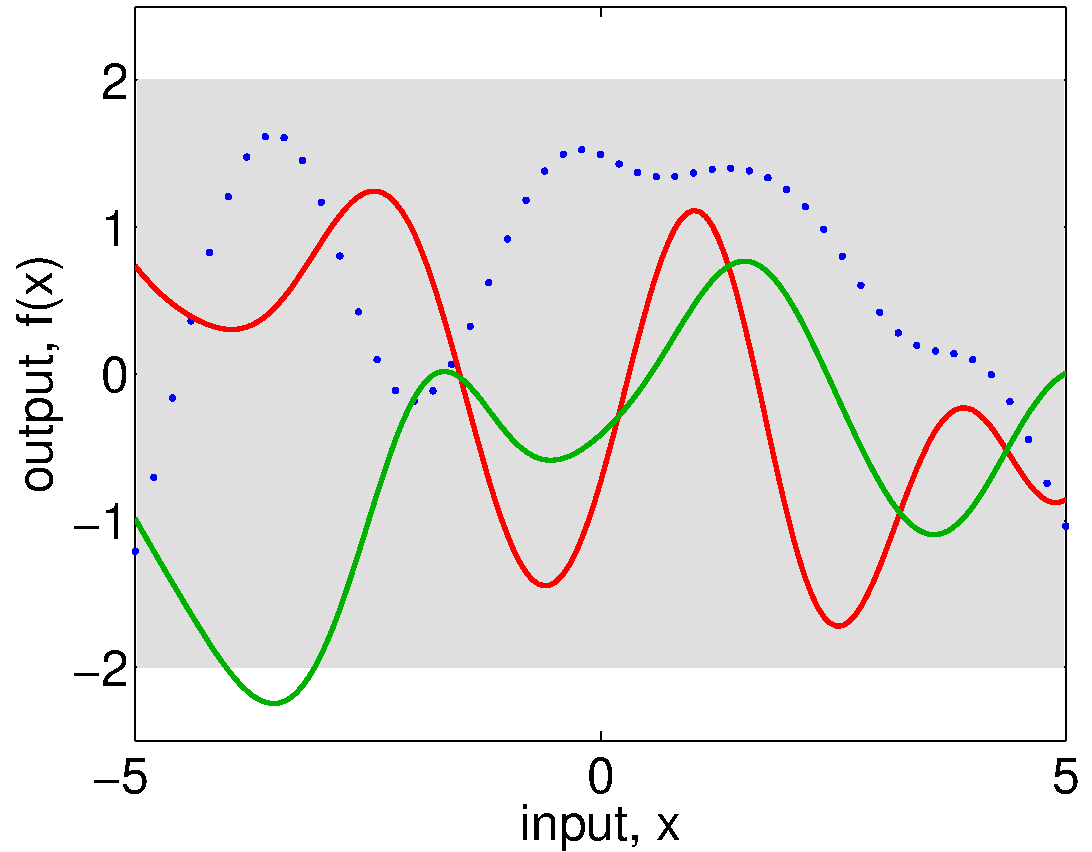
\includegraphics[width=0.45\textwidth]{priorpost} &
{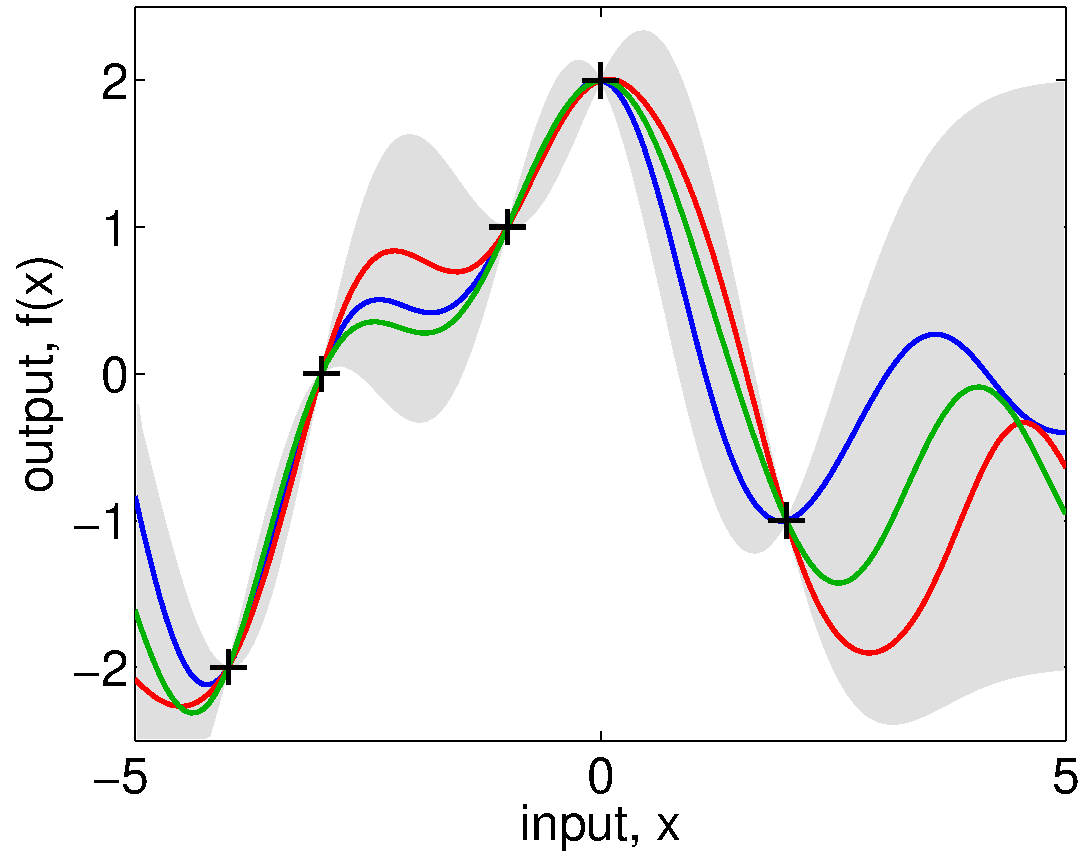
\includegraphics[width=0.45\textwidth]{priorpost1}}
\end{tabular}
\end{center}

Predictive distribution:
\[
\begin{split}
p(y_*|x_*,{\bf x},{\bf y})\;\sim\;{\cal N}\big(&{\bf k}(x_*,{\bf x})^\top
[K+\sigma_{\rm noise}^2I]^{-1}{ \bf y},\\
&k(x_*,x_*)+\sigma_{\rm noise}^2 - {\bf k}(x_*,{\bf x})^\top 
[K+\sigma_{\rm noise}^2I]^{-1}{\bf k}(x_*,{\bf x})\big)
\end{split}
\]
\end{frame}

\begin{frame}
\frametitle{Some interpretation}

Recall our main result:
\[
\begin{split}
f_*|x_*,\bfx,{\bf y}\;\sim\; {\cal N}\big(&\Blue{K(x_*,\bfx)
[K(\bfx,\bfx)+\sigma_\mathrm{noise}^2I]^{-1}{\bf y},}\\
&\Red{K(x_*,x_*)-K(x_*,\bfx)[K(\bfx,\bfx)+\sigma_\mathrm{noise}^2I]^{-1}K(\bfx,x_*)}\big).
\end{split}
\]
The \Blue{mean} is linear in two ways:
\[
\mu(x_*)\;=\;\Blue{k(x_*,\bfx)[K(\bfx,\bfx)+\sigma_\mathrm{noise}^2I]^{-1}{\bf y}}
\;=\;\sum_{n=1}^N\beta_n y_n\;=\;
\sum_{n=1}^N\alpha_nk(x_*,x_n).
\]
The last form is most commonly encountered in the kernel literature.

The \Red{variance} is the difference between two terms:
\[
V(x_*)\;=\;\Red{k(x_*,x_*)-{\bf k}(x_*,\bfx)
[K(\bfx,\bfx)+\sigma_\mathrm{noise}^2I]^{-1}{\bf k}(\bfx,x_*)},
\]
the first term is the \emph{prior variance}, from which we subtract
a (positive) term, telling how much the data $\bfx$ has
explained.\\
Note, that the variance is independent of the observed
outputs ${\bf y}$.
\end{frame}


\end{document}
